\documentclass[11pt,a4paper]{article}
\usepackage[margin=2.5cm]{geometry}
\usepackage{graphicx}
\title{Labwork 6: Map}
\author{Duong Tan Binh \\ Student ID: 2540007}
\date{}
\begin{document}
\maketitle
\section{Lab 6a: Binarization}
I use the grayscale image from Lab 4 and set the threshold to 128.
Each thread writes 0 below the threshold and 1 otherwise.
I multiply these values by 255 only when saving the black-and-white image.

\section{Lab 6b: Brightness}
I add 40 to make the image brighter and subtract 40 to make it darker.
I keep the result between 0 and 255 so that values do not wrap around.

\section{Lab 6c: Blending}
The second image is a horizontal flip of the first image, so both have
the same size. I use weight 0.5: each output pixel is half of each input.
The fractional part is dropped when storing the result as an integer.

\section{Block sizes}
I test 8 by 8, 16 by 16 and 32 by 32 blocks. Each thread handles one pixel.
The times below include both input transfers, all four operations
(binary, brighter, darker and blend), and their output transfers.
The kernels run once before timing. Each configuration is measured once.

\begin{verbatim}
Block size: (8, 8)
Total time: 1.248 ms
Block size: (16, 16)
Total time: 0.761 ms
Block size: (32, 32)
Total time: 0.752 ms
\end{verbatim}
The 32 by 32 block is slightly faster than 16 by 16 in this run.
All block sizes give the same outputs.

\newpage
\section{Images}
\begin{center}
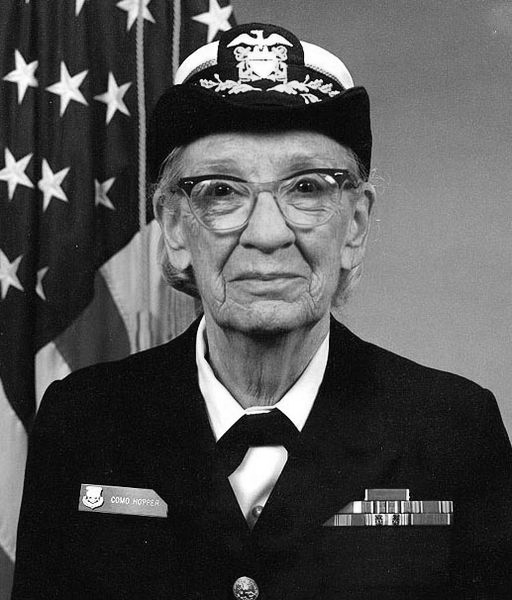
\includegraphics[width=0.35\textwidth]{input1.png}
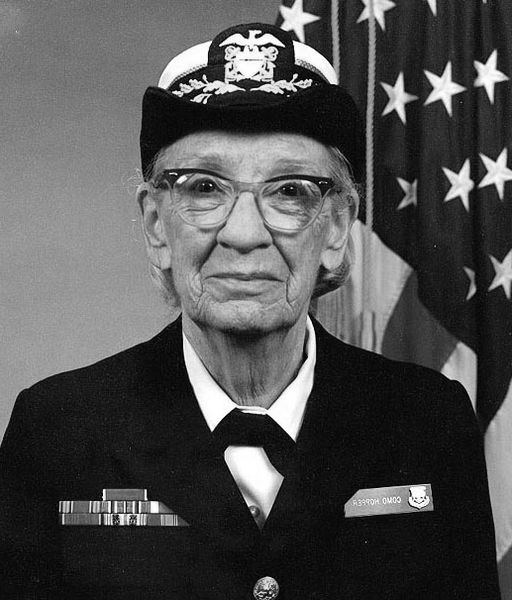
\includegraphics[width=0.35\textwidth]{input2.png}
\end{center}
Input 1 and input 2.
\begin{center}
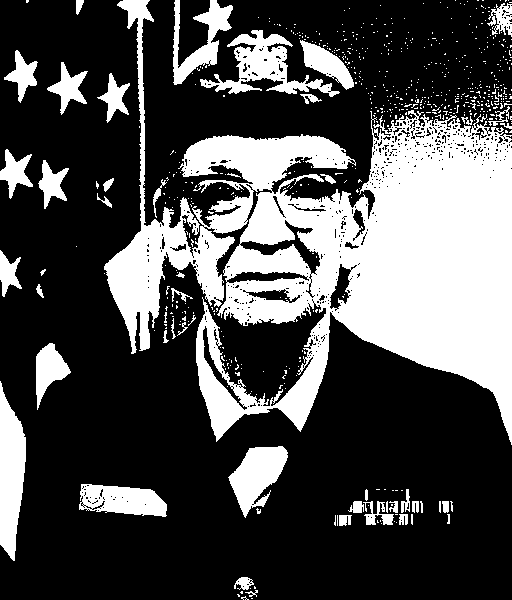
\includegraphics[width=0.22\textwidth]{binary.png}
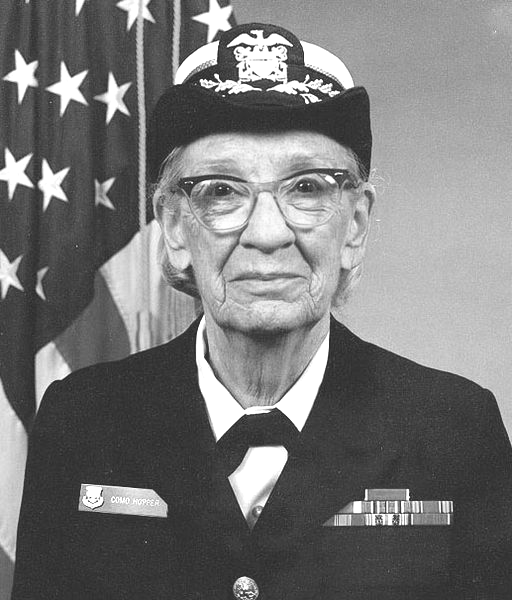
\includegraphics[width=0.22\textwidth]{bright.png}
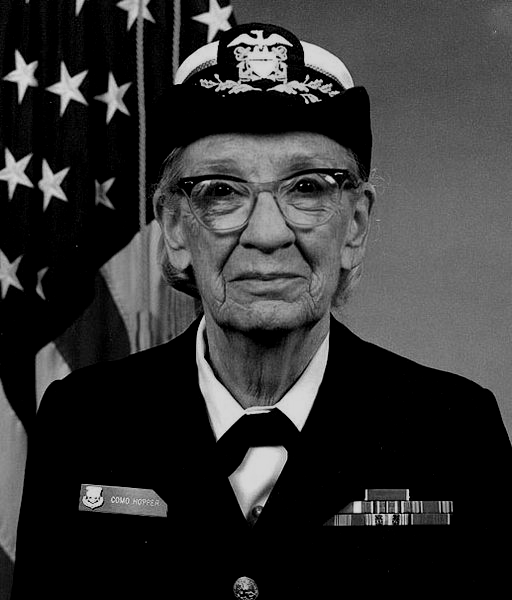
\includegraphics[width=0.22\textwidth]{dark.png}
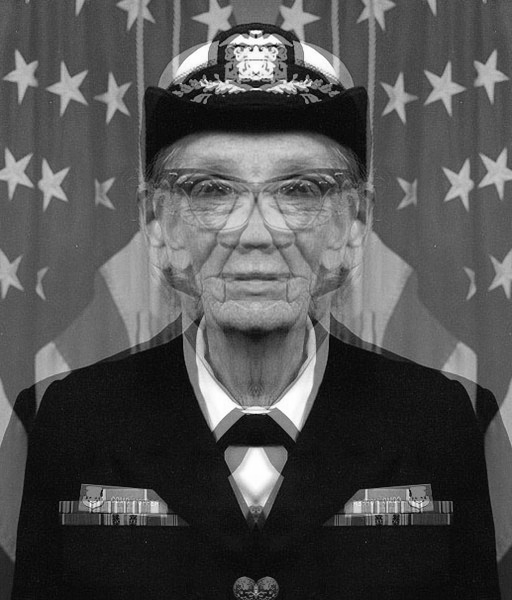
\includegraphics[width=0.22\textwidth]{blend.png}
\end{center}
From left to right: binary, brighter, darker and blended.

\end{document}
